\documentclass[border=2pt]{standalone}
\usepackage{tikz}
\usetikzlibrary{arrows.meta,positioning,shapes.geometric}

\begin{document}
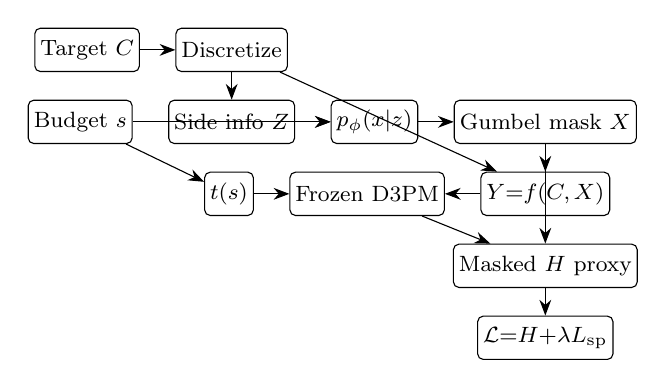
\begin{tikzpicture}[
  node distance=0.35cm and 0.45cm,
  box/.style={draw, rounded corners=2pt, align=center, font=\footnotesize,
              minimum height=0.55cm, inner sep=2pt},
  arr/.style={-{Stealth[length=2mm]}, font=\scriptsize}
]
  \node[box] (c) {Target $C$};
  \node[box, right=of c] (disc) {Discretize};
  \node[box, below=of disc] (z) {Side info $Z$};
  \node[box, left=of z] (s) {Budget $s$};
  \node[box, right=of z] (masknet) {$p_\phi(x|z)$};
  \node[box, right=of masknet] (x) {Gumbel mask $X$};
  \node[box, below=of x] (y) {$Y{=}f(C,X)$};
  \node[box, left=of y] (d3pm) {Frozen D3PM};
  \node[box, left=of d3pm] (tmap) {$t(s)$};
  \node[box, below=of y] (ent) {Masked $H$ proxy};
  \node[box, below=of ent] (loss) {$\mathcal{L}{=}H{+}\lambda L_{\mathrm{sp}}$};

  \draw[arr] (c) -- (disc);
  \draw[arr] (disc) -- (z);
  \draw[arr] (disc) -- (y);
  \draw[arr] (s) -- (masknet);
  \draw[arr] (z) -- (masknet);
  \draw[arr] (masknet) -- (x);
  \draw[arr] (x) -- (y);
  \draw[arr] (s) -- (tmap);
  \draw[arr] (tmap) -- (d3pm);
  \draw[arr] (y) -- (d3pm);
  \draw[arr] (d3pm) -- (ent);
  \draw[arr] (x) -- (ent);
  \draw[arr] (ent) -- (loss);
\end{tikzpicture}
\end{document}
